% This file was created by tikzplotlib v0.9.2.
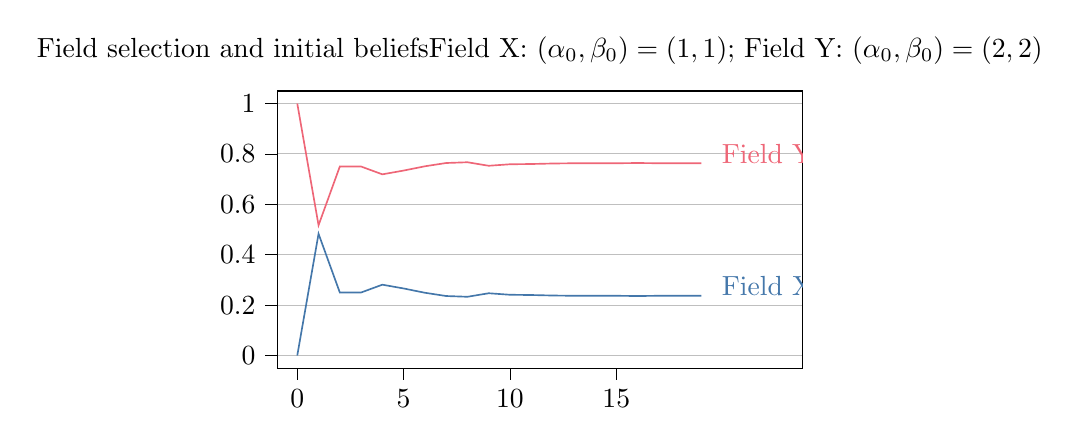
\begin{tikzpicture}

\definecolor{color0}{rgb}{0.266666666666667,0.466666666666667,0.666666666666667}
\definecolor{color1}{rgb}{0.933333333333333,0.4,0.466666666666667}

\begin{axis}[
height=5.101085673964669cm,
tick align=outside,
tick pos=left,
title={Field selection and initial beliefs \\ Field X: \(\displaystyle (\alpha_0, \beta_0)=(1, 1)\); Field Y: \(\displaystyle (\alpha_0, \beta_0)=(2, 2)\)},
width=8.25373cm,
x grid style={white!69.0196078431373!black},
xmin=-0.95, xmax=23.75,
xtick style={color=black},
xtick={0,5,10,15},
xticklabels={\(\displaystyle 0\),\(\displaystyle 5\),\(\displaystyle 10\),\(\displaystyle 15\)},
ymajorgrids,
ymin=-0.05, ymax=1.05,
ytick style={color=black},
ytick={0,0.2,0.4,0.6,0.8,1},
yticklabels={\(\displaystyle 0\),\(\displaystyle 0.2\),\(\displaystyle 0.4\),\(\displaystyle 0.6\),\(\displaystyle 0.8\),\(\displaystyle 1\)}
]
\addplot [semithick, color0]
table {%
0 0
1 0.483
2 0.25
3 0.25
4 0.281
5 0.266
6 0.249
7 0.236
8 0.233
9 0.247
10 0.241
11 0.24
12 0.238
13 0.237
14 0.237
15 0.237
16 0.236
17 0.237
18 0.237
19 0.237
};
\addplot [semithick, color1]
table {%
0 1
1 0.517
2 0.75
3 0.75
4 0.719
5 0.734
6 0.751
7 0.764
8 0.767
9 0.753
10 0.759
11 0.76
12 0.762
13 0.763
14 0.763
15 0.763
16 0.764
17 0.763
18 0.763
19 0.763
};
\draw (axis cs:19.5,0.237) node[
  anchor=base west,
  text=color0,
  rotate=0.0
]{Field X};
\draw (axis cs:19.5,0.763) node[
  anchor=base west,
  text=color1,
  rotate=0.0
]{Field Y};
\end{axis}

\end{tikzpicture}
